\documentclass[a4paper]{report}

\usepackage[latin1]{inputenc} % accents
\usepackage[T1]{fontenc}      % caract�res fran�ais
\usepackage[francais]{babel}  % langue
\usepackage{graphicx}         % images
\usepackage{verbatim}         % texte pr�format�
\usepackage{listings}
\usepackage[]{algorithm2e}
\usepackage[margin=0.8in]{geometry}
\usepackage[table]{xcolor}

\addto\captionsfrancais{% Replace "english" with the language you use
  \renewcommand{\contentsname}%
    {Sommaire}%
}

\begin{document}

\begin{titlepage}
\fontfamily{phv}\selectfont
\vspace*{\stretch{1}}
\begin{flushright}\LARGE
Accassias
\end{flushright}
\hrule
\begin{flushleft}\huge\bfseries
User Manual
\end
{flushleft}
\vspace*{\stretch{2}}
\begin{center}
Eric Therond
\end{center}
\end{titlepage}

\tableofcontents

\chapter{Introduction}

  \section{Pr�sentation d'Accassias}

    \subsection{Description g�n�rale}
\textit{Accassias} est un outil pour l'aide � l'analyse statique de codes sources. Il est �crit dans un but d'apprentissage, � la fois l'�tude de la programmation en \textit{C++} et la recherche automatis�e de d�fauts logiciel.

  \newpage

\chapter{Utilisation}

On execute ici le programme example1.aca �crit en langage \textit{Accassias}
\newline
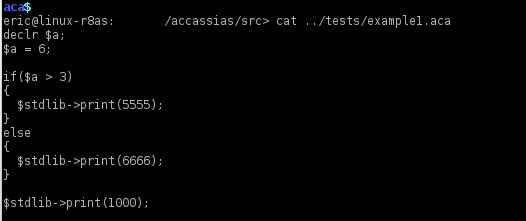
\includegraphics[scale=1]{cat_example1.png}
\vspace{5mm}
\newline
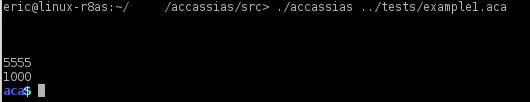
\includegraphics[scale=1]{load_accassias.png}

  \section{Calcul de l'arbre de syntaxe abstraite}
On lance l'�criture de l'ast au format dot � l'aide de l'appel � la m�thode \begin{verbatim}$ast->dot("dotexample1.dot");\end{verbatim}
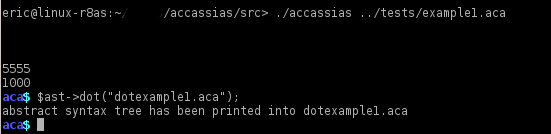
\includegraphics[scale=1]{ast_cmd_example1.png}
\vspace{5mm}
\newline
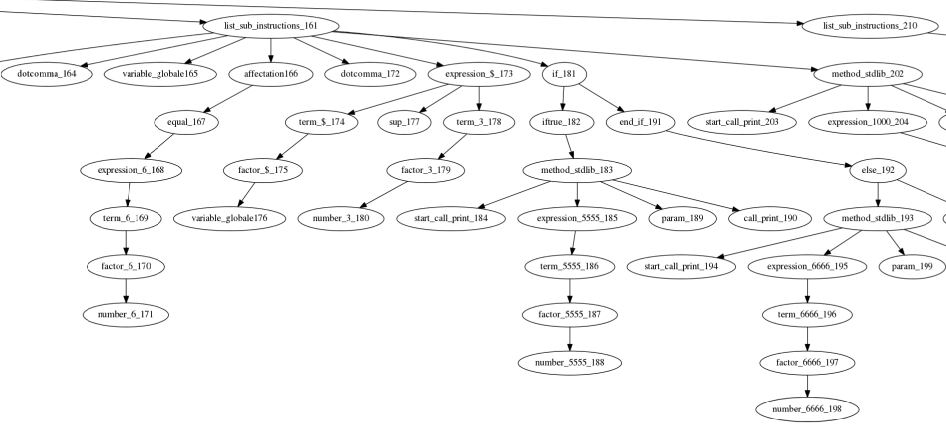
\includegraphics[scale=0.7]{ast_example1.png}

  \section{Calcul du three address code}
On affiche le three address code � l'aide de l'appel � la m�thode \begin{verbatim}$stdlib->system("show_tac");\end{verbatim}
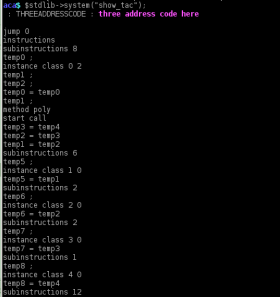
\includegraphics[scale=1]{tac_example1.png}

  \section{Calcul du control flow graph}
On calcul le control flow graph � l'aide de l'appel � la m�thode \begin{verbatim}$cfg->compute();\end{verbatim}

\includegraphics[scale=1]{cfg_compute_cmd_example1.png}
\vspace{5mm}
\newline
On �crit le control flow graph au format dot � l'aide de l'appel � la m�thode \begin{verbatim}$cfg->dot("cfgexample1.dot");\end{verbatim}

\includegraphics[scale=1]{cfg_cdot_cmd_example1.png}
\vspace{5mm}
\newline
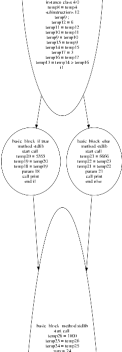
\includegraphics[scale=1]{cfg_example1.png}

  \section{Calcul du code machine}
On affiche le code machine � l'aide de l'appel � la m�thode \begin{verbatim}$stdlib->system("show_code");\end{verbatim}
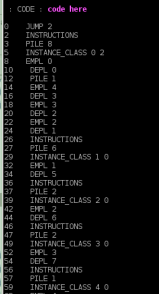
\includegraphics[scale=1]{code_example1.png}

  \section{Affichage de l'�tat de la machine virtuelle}
On affiche l'�tat de la machine virtuelle � l'aide de l'appel � la m�thode \begin{verbatim}$stdlib->system("show_statevm");\end{verbatim}
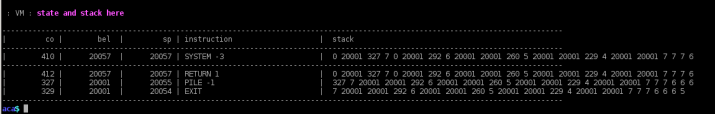
\includegraphics[scale=1]{statevm_example1.png}

% \listoffigures
% \listoftables

\end{document}
